\usepackage{pgfplots}
\usepackage{graphicx}
\usepackage{amsmath}


\section{Method}

\subsection{Similarity Judgment Criteria}

\begin{figure}[h]
    \centering
    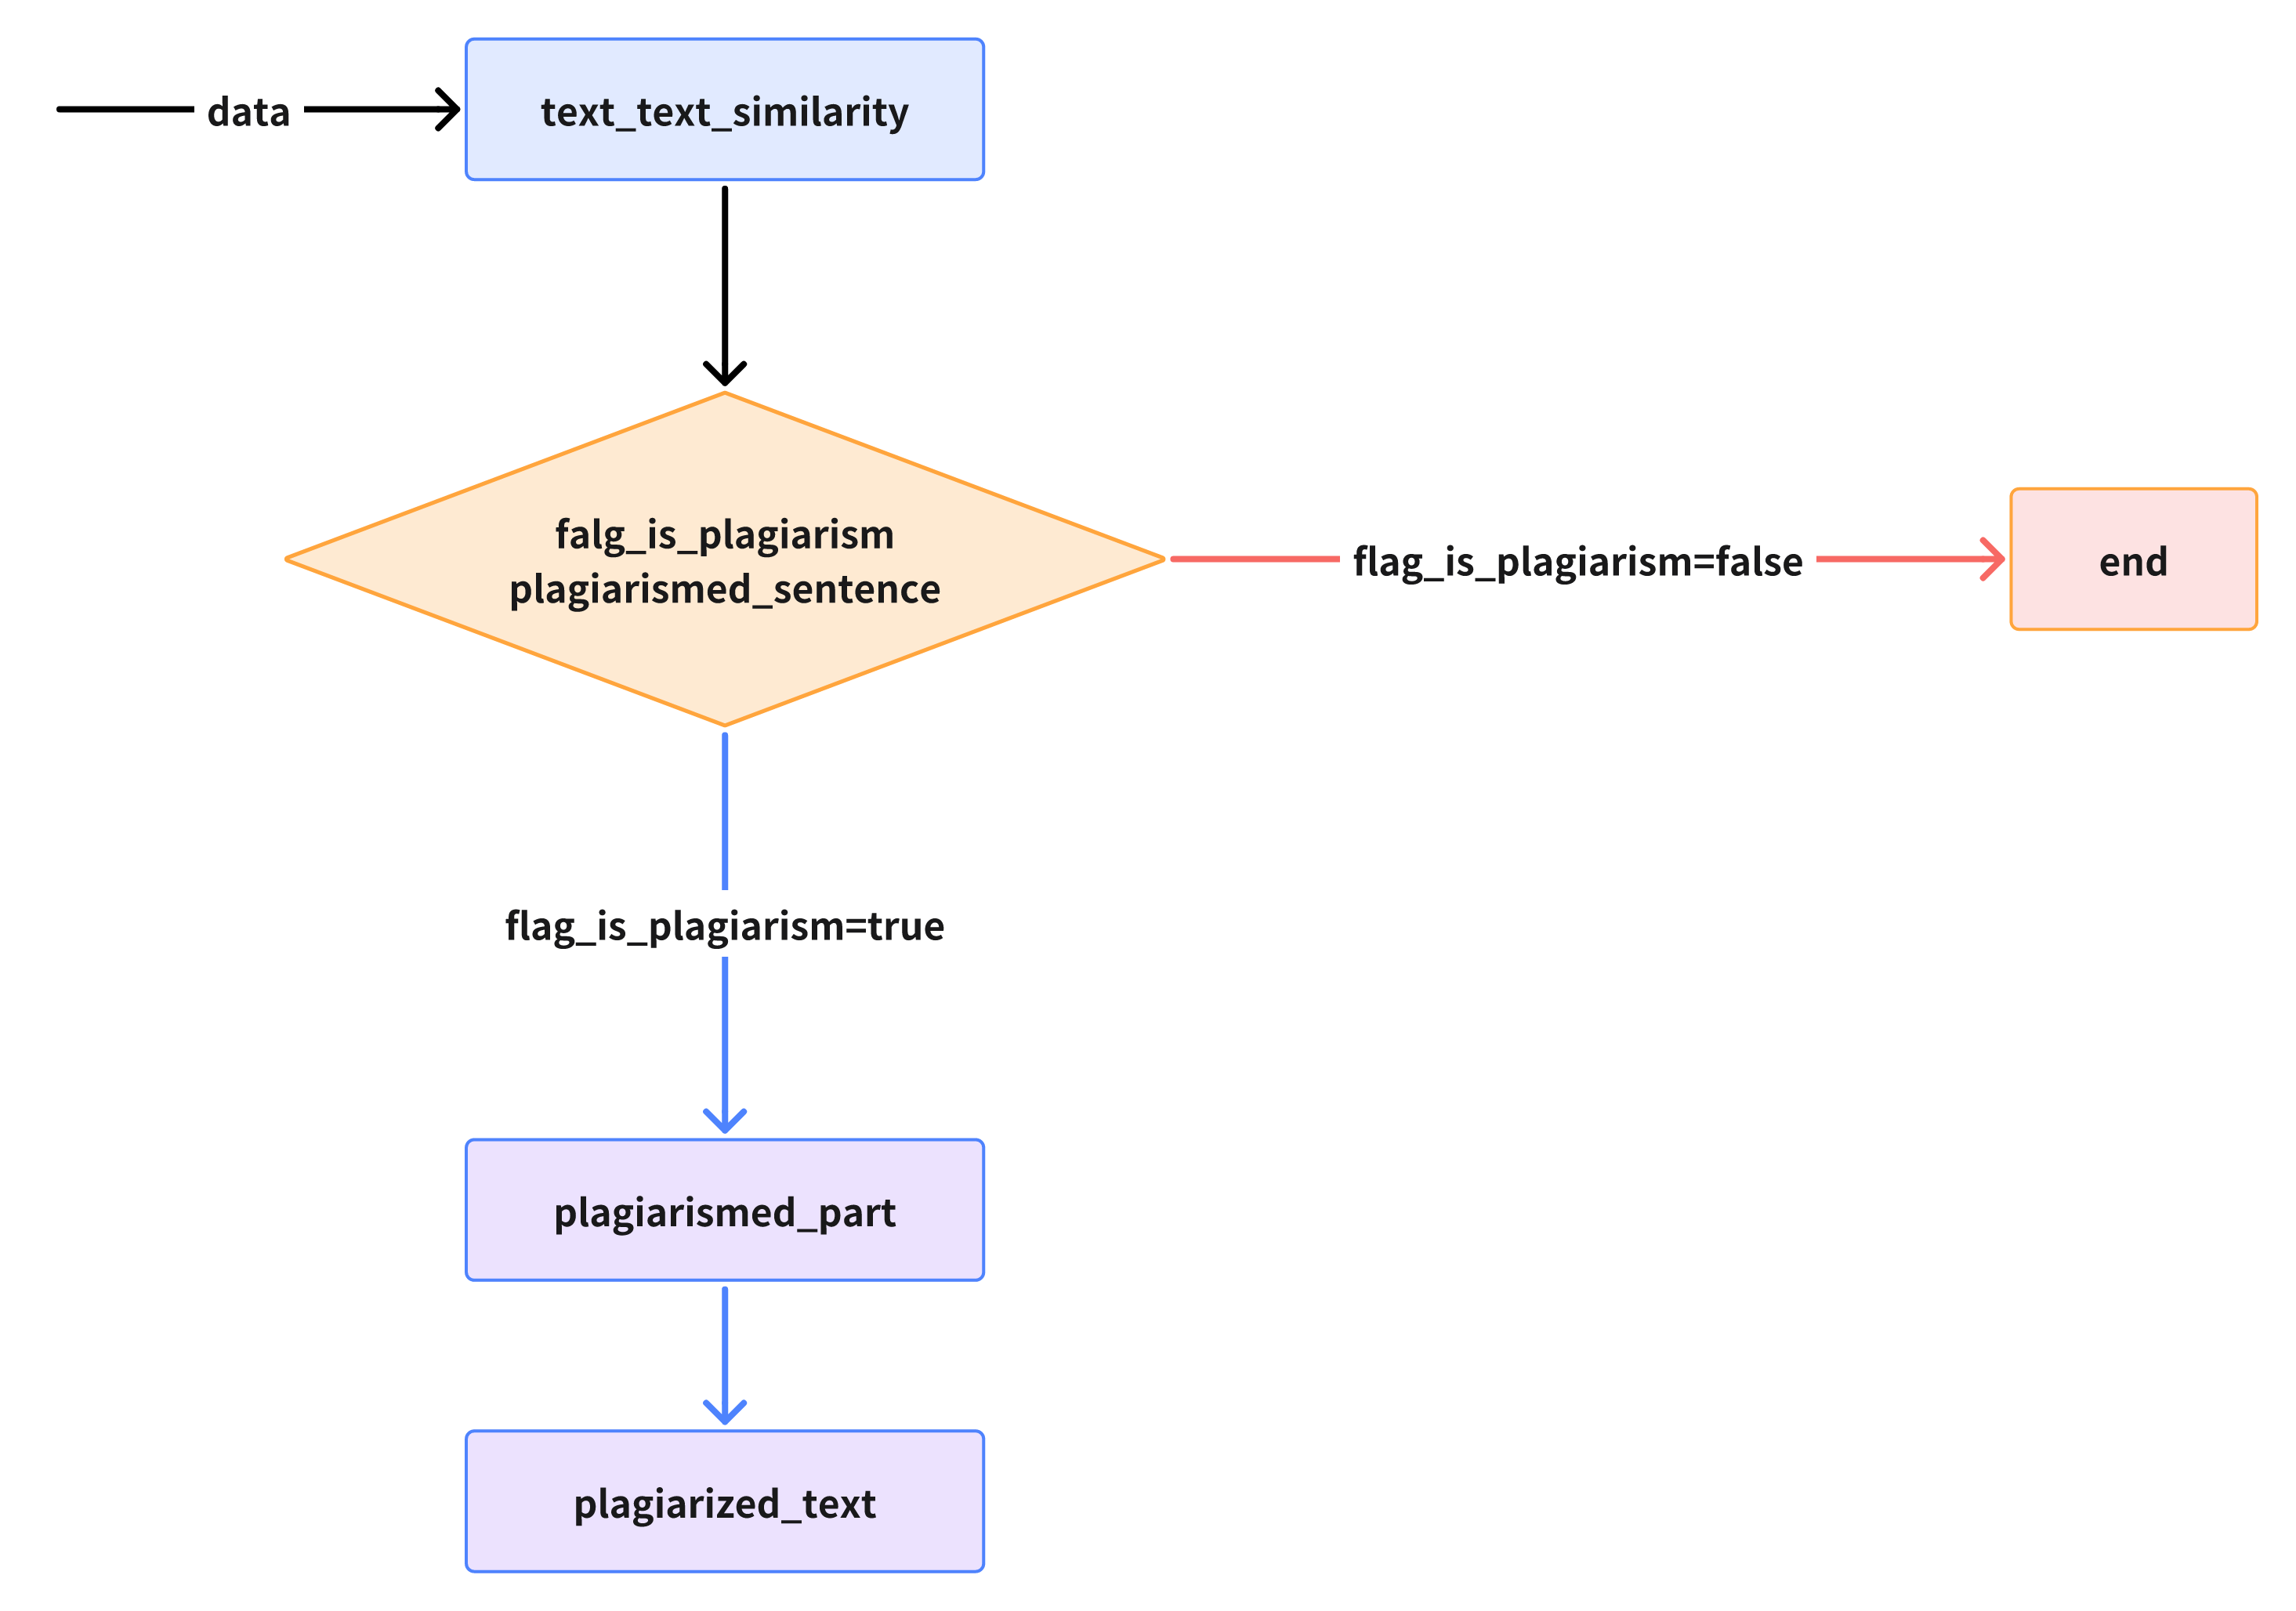
\includegraphics[width=1\linewidth]{png/system_demo.png}
    \caption{system framework}
    \label{fig:1}
\end{figure}

\subsubsection{Dot Product Similarity}
Dot Product Similarity is a common method for measuring the similarity between two vectors, especially in high-dimensional vector spaces. It calculates the similarity by computing the dot product (inner product) of two vectors.

Specifically, for two vectors \( A = (a_1, a_2, \dots, a_n) \) and \( B = (b_1, b_2, \dots, b_n) \), their dot product similarity is defined as:

\[
\text{Similarity}(A, B) = \sum_{i=1}^{n} a_i \cdot b_i
\]

In text processing or Natural Language Processing (NLP), vectors typically represent embeddings of words, sentences, or documents. By calculating the dot product of these embeddings, one can reflect the similarity between them. If the dot product of two vectors is large, it indicates that they are more similar in some feature space, meaning their similarity is higher.

\subsubsection{Cosine Similarity}
Cosine Similarity is a method for measuring the similarity of two vectors in terms of their direction, widely used in fields like text analysis and information retrieval. It determines the similarity between two vectors by calculating the cosine of the angle between them, without considering their magnitude.

Specifically, for two vectors \( A = (a_1, a_2, \dots, a_n) \) and \( B = (b_1, b_2, \dots, b_n) \), the cosine similarity is defined as:

\[
\text{Cosine Similarity}(A, B) = \frac{A \cdot B}{\|A\| \|B\|}
\]

where:
- \( A \cdot B \) is the dot product of vectors \( A \) and \( B \),
- \( \|A\| \) and \( \|B\| \) are the magnitudes (or lengths) of vectors \( A \) and \( B \), calculated as: 
  \[
  \|A\| = \sqrt{a_1^2 + a_2^2 + \dots + a_n^2}
  \]
  \[
  \|B\| = \sqrt{b_1^2 + b_2^2 + \dots + b_n^2}
  \]

The cosine similarity value ranges from -1 to 1:
\begin{itemize}
    \item \textbf{When the cosine similarity is 1}: It indicates that the directions of the two vectors are exactly the same.
    \item \textbf{When the cosine similarity is 0}: It indicates that the vectors are perpendicular and have completely different directions.
    \item \textbf{When the cosine similarity is -1}: It indicates that the directions of the two vectors are exactly opposite.
\end{itemize}

\subsubsection{Our Similarity Judgment Criteria}
\

During the experiment, we attempted to use two different similarity measures, but the performance of the dot product similarity was consistently poorer. This could be because the dot product similarity is sensitive to the position. In text plagiarism detection, the relative position is always crucial. A simple example is that the similarity between "This is an apple" and "An apple this is" should be high, but in dot product similarity, the similarity between these two sentences is not as high. Therefore, in this experiment, we used cosine similarity as our similarity measure.
\

We randomly generated 100 sentences similar to "This is an apple" and "An apple this is", and used two similarity evaluation methods to determine the accuracy of plagiarism detection. The results are as follows.
\[
\begin{array}{c|c}
\text{Method} & \text{Accuracy} \\
\hline
\text{Dot Product Similarity} & 74.48\% \\
\text{Cosine Similarity} & 85.69\% \\
\end{array}
\]

\subsection{Similarity evaluation}
\

Similarity evaluation is carried out based on the following three steps:
\subsubsection{Text Vectorization:}
\

The SentenceTransformer model, which is based on the Transformer architecture, is used here. SentenceTransformer focuses on mapping sentences or paragraphs to embedding vectors. Each sentence is transformed into a fixed-size high-dimensional vector, where each element of the vector represents different features or semantic information of the text. The position of the sentence in the high-dimensional space ensures that semantically similar sentences are closer to each other, while sentences with more semantic differences are farther apart. By doing this, different sentences or text segments are mapped to vector space, and we then compare these vectors to assess their similarity.

\subsubsection{Normalization:}
\

For each text's embedding vector, we apply the following formula for normalization:  
\[
\text{normalized\_embeddings} = \frac{\text{embeddings}}{\|\text{embeddings}\|}
\]  
The normalized embedding vectors have a length of 1, so during subsequent calculations, we focus only on the direction of the vector. Therefore, the similarity between texts is determined by their position in semantic space, independent of the length or complexity of the text itself.

\subsubsection{Similarity Calculation (Cosine Similarity):}
\

In a scenario with multiple texts, how can we identify the parts between two texts that are most likely plagiarized? To address this issue, we propose a simple yet effective method: splitting sentences. Since we can already retrieve plagiarism information between individual texts and provide a reliable quantitative metric, breaking a large problem into smaller, simpler sub-problems is always an effective approach. Specifically, the text is split into multiple sentences, and then each sentence is traversed individually. The two sentences with the highest similarity are considered the most likely plagiarized sentences. This method has the following advantages:

\subsection{Get the plagiarismed part}
\

In a scenario with multiple texts, how can we distinguish the most likely plagiarized parts between two texts? To address this issue, we propose a simple yet effective method: splitting sentences. Since we can already retrieve plagiarism information between individual texts and provide a reliable quantitative metric, breaking a large problem into smaller, simpler sub-problems is always an effective approach. This method has the following advantages:

\begin{enumerate}
    \item \textbf{High Readability}: \\
    Splitting the text into independent sentences not only simplifies the processing workflow but also improves the transparency and readability of plagiarism detection. After splitting the text by sentence, we can evaluate the similarity between each sentence and others, instead of performing a complex comparison of entire documents. This way, users can clearly see the similarity scores for each sentence and quickly identify potential plagiarized segments. This approach makes the results easier to understand and helps with subsequent analysis and validation.
    
    \item \textbf{Effective Identification of Implicit Plagiarism}: \\
    A common issue in plagiarism detection is the rearrangement of sentence order to evade detection. Traditional plagiarism detection methods may be affected by changes in sentence order, but our method avoids this problem by splitting sentences. Each sentence is evaluated independently, and relative order is ignored. Therefore, even if plagiarism is committed by rearranging sentence order, it can still be effectively detected.
    
    \item \textbf{Easy to Expand}: \\
    By splitting the text into individual sentences, our system becomes highly flexible and can handle texts of varying scales and complexities. Whether it's a short paragraph or a lengthy article, we can break it into smaller units for processing. This method also facilitates future expansion or adjustments as needed. For instance, we could further refine the similarity evaluation to the word level or incorporate more contextual information for higher-level semantic matching.
\end{enumerate}



